\section{Auswertung}
\label{sec:auswertung}

Im Anschluss werden die aufgenommenen Messwerte ausgewertet.

\subsection{Energiekalibration und Bestimmung der Vollenergienachweiswahrscheinlichkeit}
\label{sec:auswertung1}

Das aufgenommene Spektrum der Eu-152 Quelle ist in der Abbildung \ref{fig:plot1}
dargestellt. Die Anzahl der Impulse wurden für eine bessere Darstellbarkeit logarithmisch abgebildet. 

\begin{figure}[H]
    \centering
    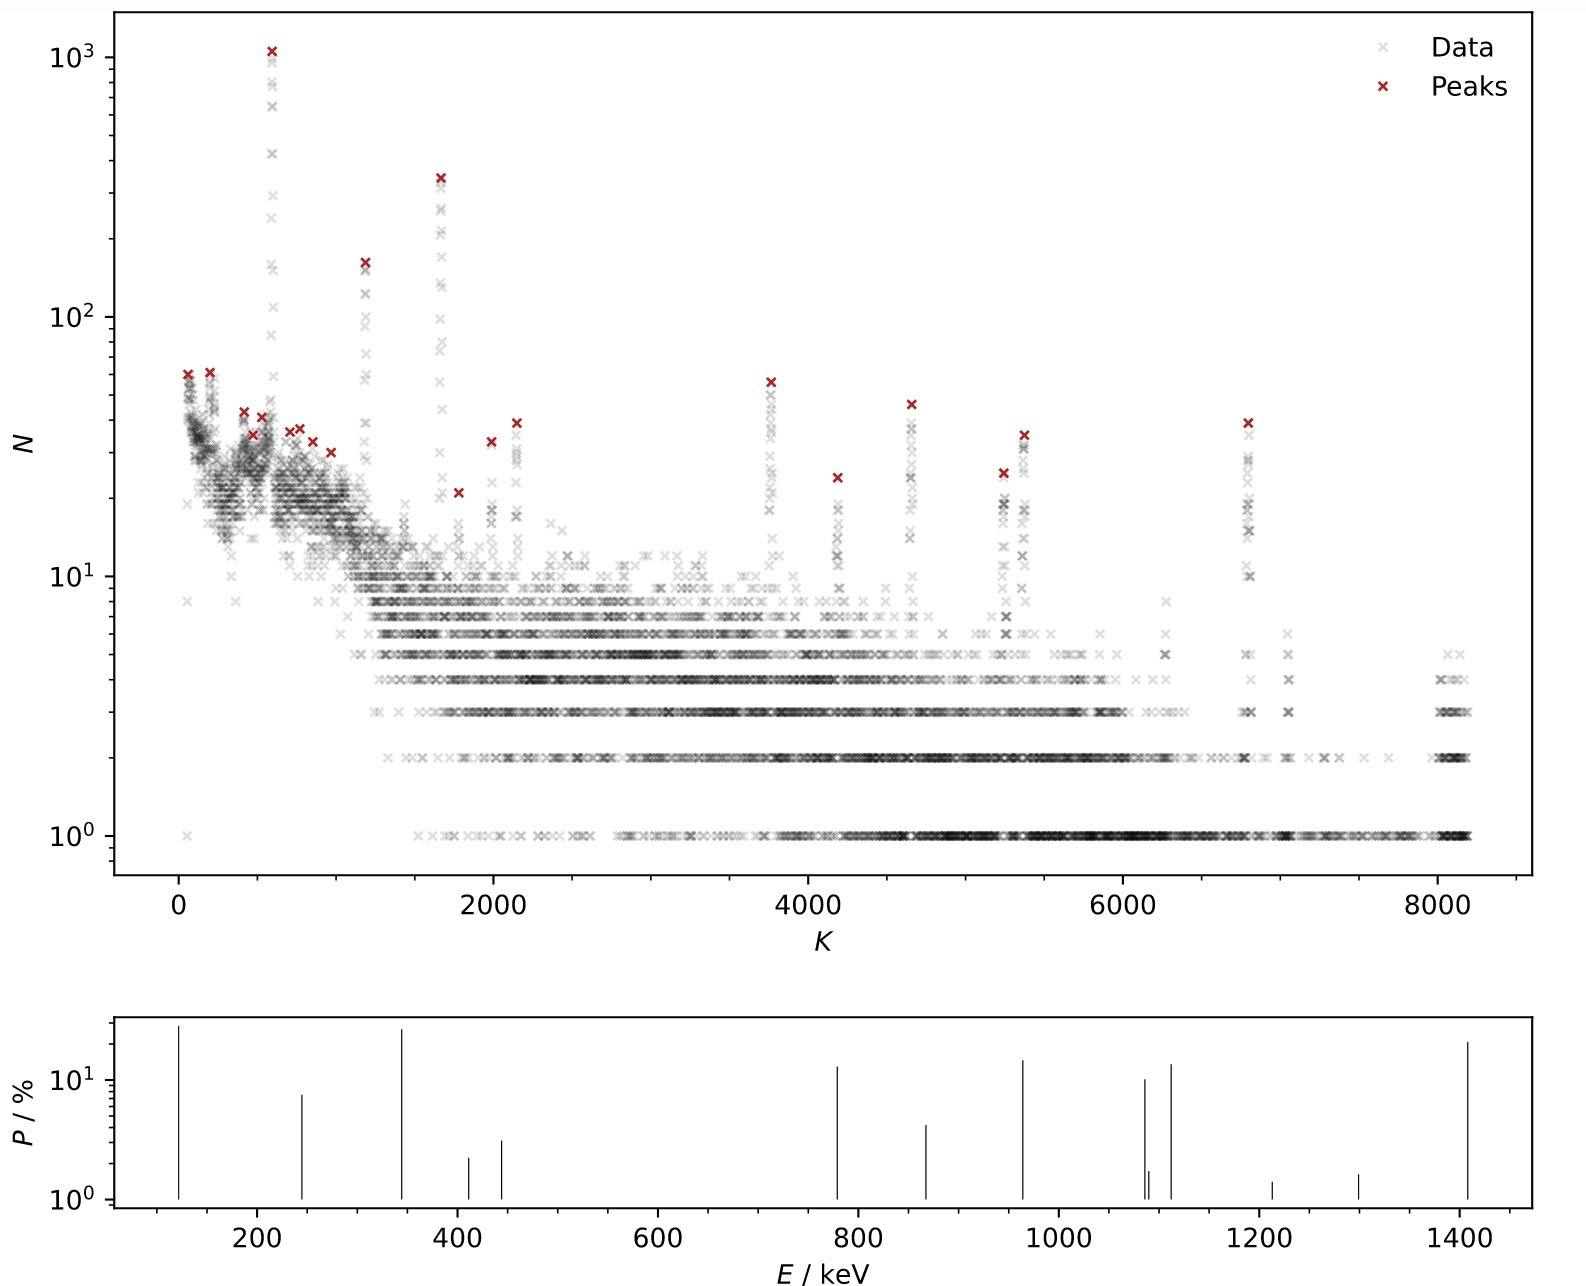
\includegraphics[width=0.9\textwidth]{content/plots/plot1.jpg}
   \caption{Gammaspektrum des Eu-152 Strahlers.}
    \label{fig:plot1}
\end{figure}

Die Photopeaks werden mit dem SciPy Paket find-peaks ermittelt und rot markiert.
Unter dem Spektrum befinden sich die Emissionsenergien des Gammastrahlers, welche zum Abgleichen verwendet werden.
Die Emissionsenergien von Eu-152 sind in der Abbildung \ref{fig:euE} gegeben.

\begin{figure}[H]
    \centering
    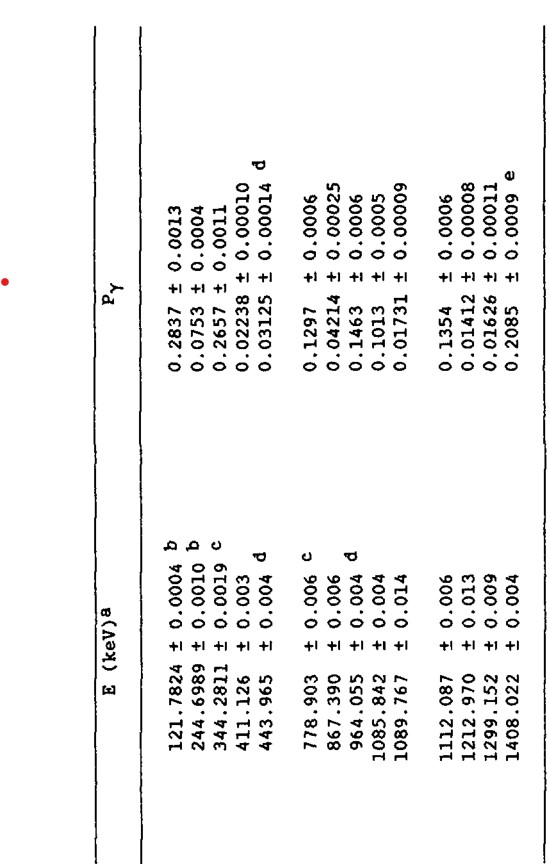
\includegraphics[angle=270,width=0.6\textwidth]{content/grafik/euenergien.jpg}
    \caption{Die Emissionsenergien von Eu-152. \cite{Kalibration}}
    \label{fig:euE}
\end{figure}

Nun werden die bereits zugeordneten Emissionsenergien gegen die Kanalnummer $K$ aufgetragen.
Anschließend wird eine lineare Ausgleichsgerade der Form 
\begin{equation*}
    a \cdot K + b
\end{equation*}
an die Werte angelegt.
Die Messwerte und die Emissionsenergien sind mit der Ausgleichsgerade in der Abbildung \ref{fig:plot2} zu sehen.

\begin{figure}[H]
    \centering
    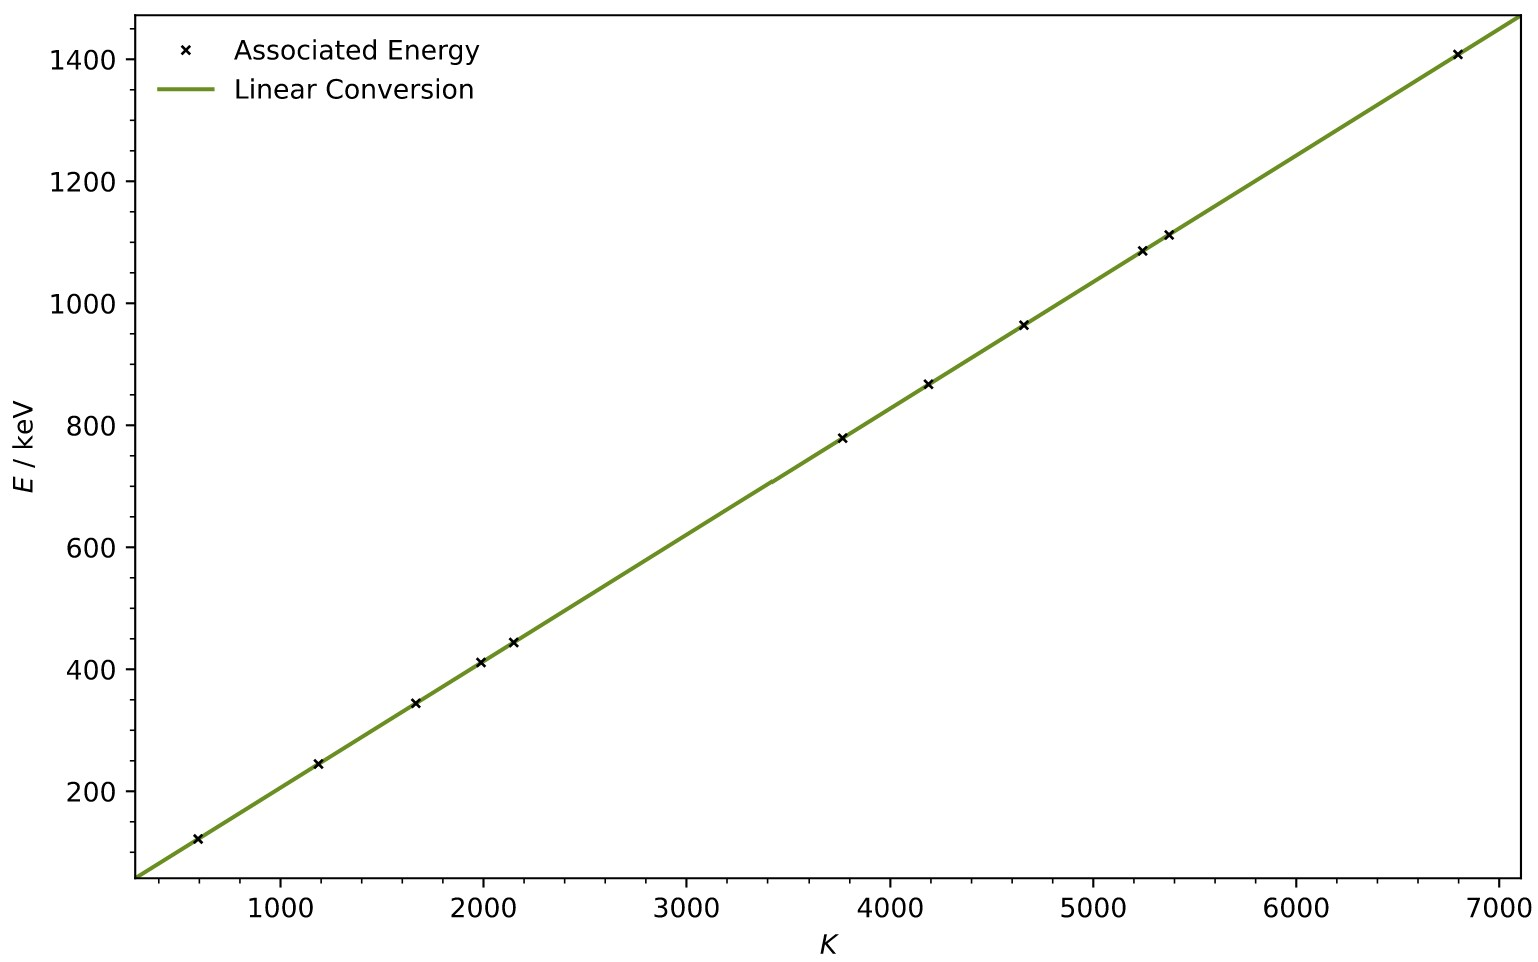
\includegraphics[width=0.8\textwidth]{content/plots/plot2.jpg}
    \caption{Ausgleichsrechnung der Energiekalibration.}
    \label{fig:plot2}
\end{figure}

Für die Parameter der Gerade ergeben sich die Werte
\begin{align*}
    a   &= \qty{0.2073+-0.0001}{\kilo\eV} \\
    b   &= \qty{-1.3399 +- 0.2191}{\kilo\eV}.
\end{align*}

Für die Energiekalibration ergibt sich demnach
\begin{equation*}
    E\left(K\right) = \qty{0.2073+-0.0001}{\kilo\eV} \cdot K + \qty{-1.3399 +- 0.2191}{\kilo\eV}.
\end{equation*}

Zur Verdeutlichung der Zuordnung der Emissionswahrscheinlichkeiten wurde das Spektrum von Eu-152 mit der Energieskala erneut erstellt und
wird in der Abbildung \ref{fig:plot3} abgebildet. Damit ist die Energiekalibration des Ge-Detektors abgeschlossen.

\begin{figure}[H]
    \centering
    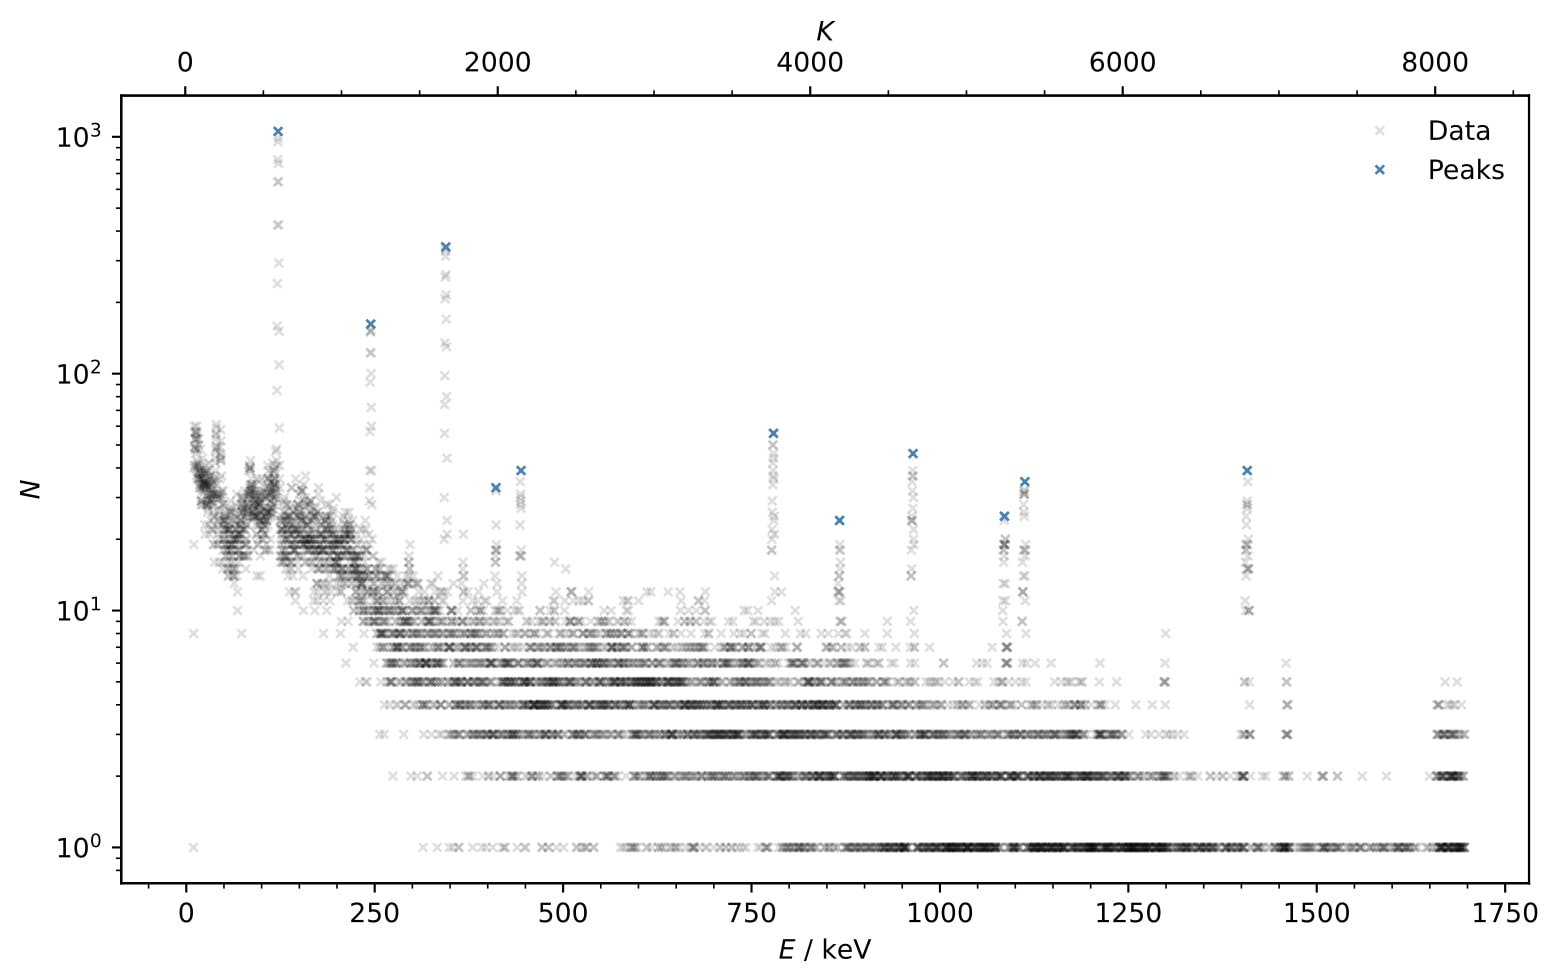
\includegraphics[width=0.8\textwidth]{content/plots/plot3.jpg}
   \caption{Gammaspektrum des Eu-152 Strahlers mit zusätzlicher Energieskala.}
   \label{fig:plot3}
\end{figure}

An die Full Energy Peaks wird jeweils eine Gaußfunktion gefitet. In der Abbildung \ref{fig:plot4} sind für den Peak bei $E$ = \qty{122}{\kilo\eV}
die Gaußkurve und die Messwerte exemplarisch abgebildet. Die Gaußfunktion hat die Form wie in Gleichung \ref{eqn:gauss}

\begin{figure}[H]
    \centering
    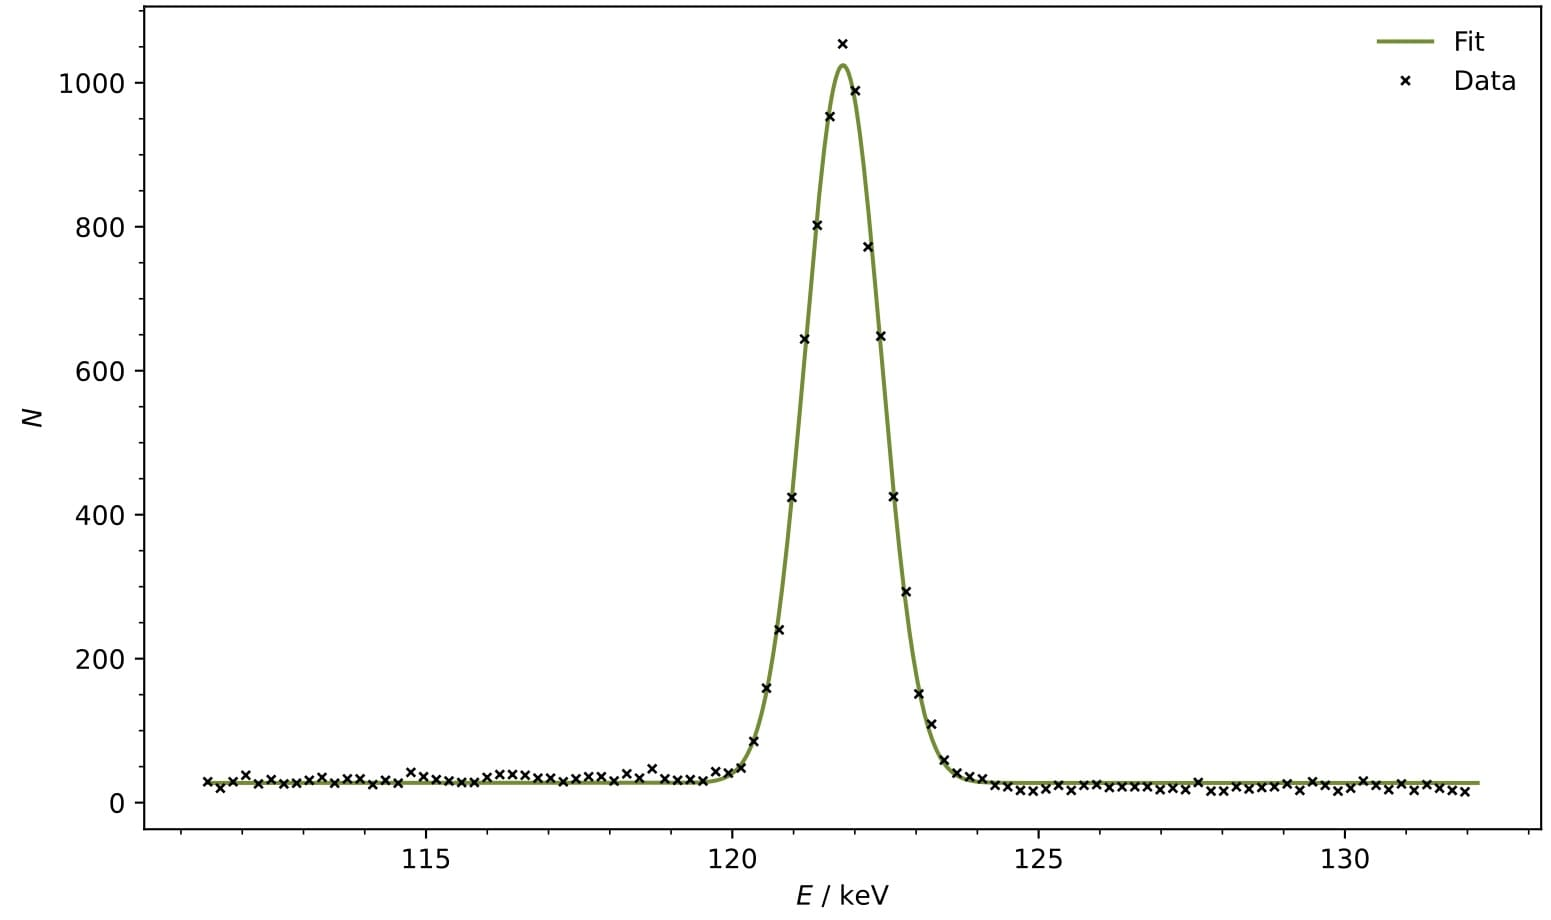
\includegraphics[width=0.8\textwidth]{content/plots/plot4.jpg}
   \caption{Fit einer Gaußkurve an einem Full Energy Peak für $E$ = \qty{122}{\kilo\eV} des Eu-152 Spektrums.}
   \label{fig:plot4}
\end{figure}

Es ist so möglich die Gesamtanzahl der Impulse pro Peak zu bestimmen. Dies ist notwendig zur weiteren Berechnung der Vollenergienachweiswahrscheinlichkeit.
Anhand des Fits kann auch der Hintergrund als konstant modelliert und durch subtraktion kompensiert werden.

Die Vollenergienachweiswahrscheinlichkeit wird mit der Gleichung 
\begin{equation*}
    Q = \frac{N}{AWt} \cdot \frac{4\pi}{\Omega}
\end{equation*}
bestimmt. $W$ Gibt die Emissionswahrscheinlichkeit an, $A$ enspricht der Aktivität der Probe am Messtag (22.04.2024) und $t$
ist die Zeitspanne, über die gemessen wird. Wie im Abschnitt \ref{sec:durchführung} nachzulesen, wurde über einen Zeitraum von ungefähr \qty{2700}{\second} gemessen.
Zur Bestimmung der Aktivität der Probe wird das Zerfallsgesetzt gemäß
\begin{equation*}
    N(t) = N_0 \exp(-\lambda t)
\end{equation*}
nach $t$ abgeleitet. Daraus folgt der Zusammenhang für die aktuelle Aktivität der Probe
\begin{equation*}
    A(t) = A_0 \exp(-\lambda t).
\end{equation*}

Die Aktivität am 01.10.2000 und die Halbwertszeit von Eu-152 sind geben durch
\begin{align*}
    A_0     &= \qty{4130+-60}{\becquerel} \\
    T_{\frac{1}{2}} &= \qty{4934}{\day}.
\end{align*}

Für den Tag der Messung (22.04.2024) ergibt sich damit eine Aktivität von
\begin{equation*}
    A = \qty{1233+-18}{\becquerel}.
\end{equation*}

Abschließen muss  der Raumwinkelanteil $\Omega$ berechnet werden und zwar anhand der Gleichung
\begin{equation*}
    \Omega = \frac{1}{2} \left(1- \frac{a}{\sqrt{a^2+r^2}}\right).
\end{equation*}

Dabei bezeichnet $a$ den Abstand der Probe zum Detektor, dieser beträgt in Summe \qty{85}{\milli\meter}.
Der Radius $r$ des zylinderförmigen Ge-Detektors entspricht \qty{22.5}{\milli\meter}.
Für den Raumwinkelanteil ergibt sich ein Wert von \num{0.01665}.
Nun können die berechneten Werte für die Vollenergienachweiswahrscheinlichkeit $Q$ mit den zugehörigen Energien in einem Diagramm
aufgetragen werden. Dies ist in der Abbildung \ref{fig:plot5} gezeigt.

\begin{figure}[H]
    \centering
    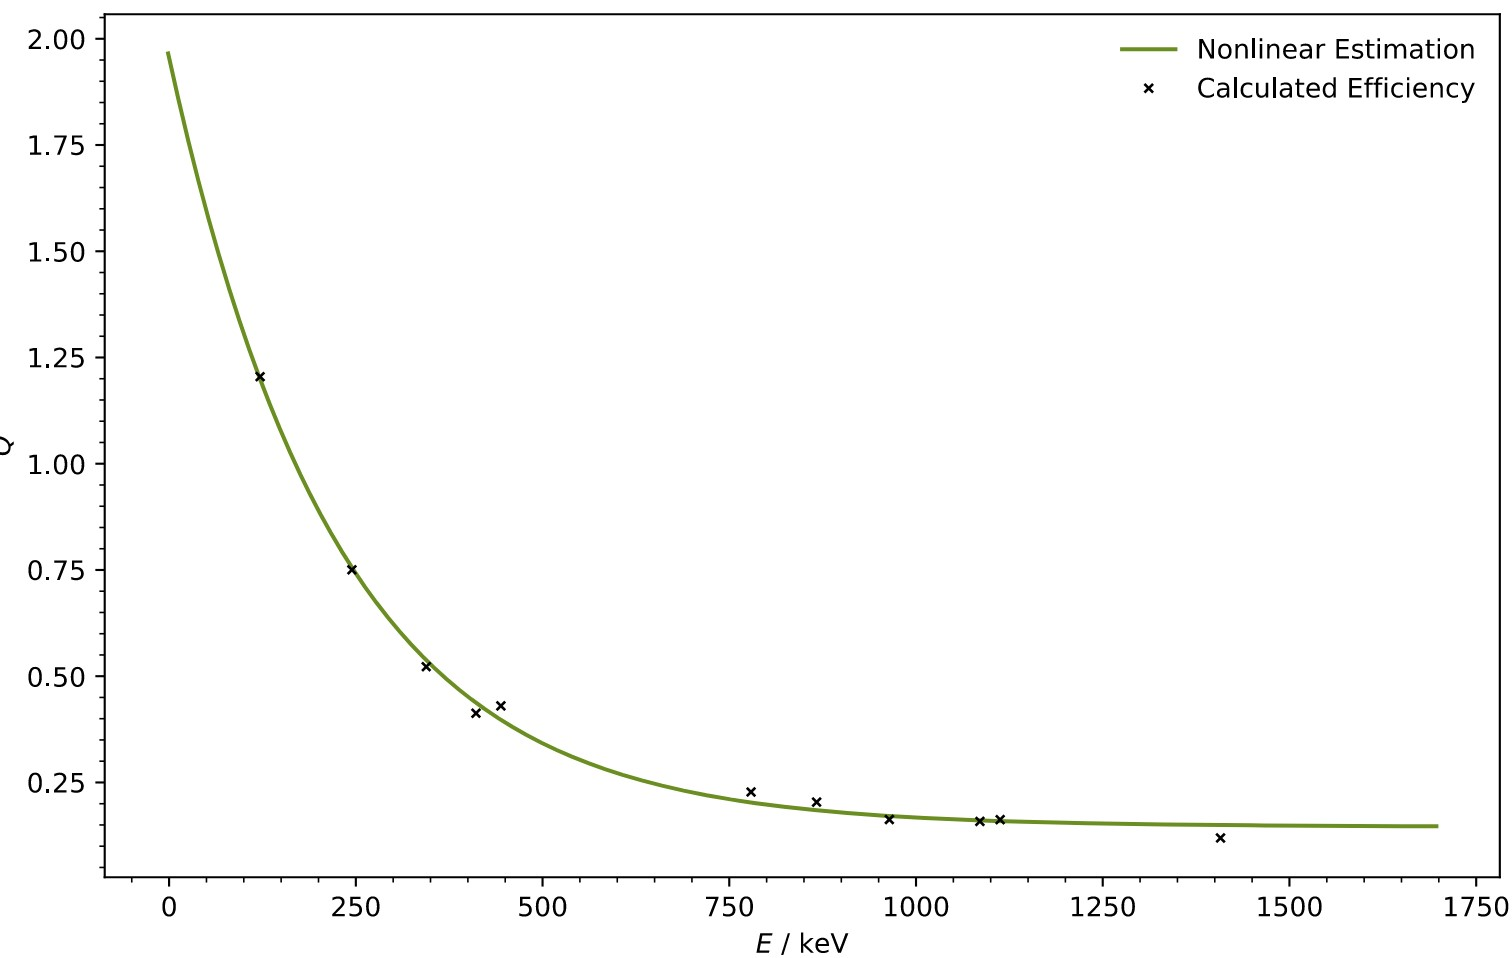
\includegraphics[width=0.8\textwidth]{content/plots/plot5.jpg}
   \caption{Die Effizienz des hochreinen Geermanium Detektors in Abhängigkeit der Energie.}
   \label{fig:plot5}
\end{figure}

Der Fit in der Abbildung \ref{fig:plot5} wurde mit einer Funktion der Form 
\begin{equation*}
    a \cdot b^x + c
\end{equation*}
an die Messwerte angelegt.
Für die Parameter ergeben sich die Werte
\begin{align*}
    a   &= \num{1.8087 +- 0.0643} \\
    b   &= \num{0.9956 +- 0.0002} \\
    c   &= \num{0.1461 +- 0.0114}.
\end{align*}
Dabei ist zu beachten, dass $Q$ einheitenlos ist. 

Anschließend wird das anfängliche Spektrum von Eu-152 mit der Funktion der Effektiviät korrigiert.
Das Resulatat ist in der Abbildung \ref{fig:plot6} dargestellt.

\begin{figure}[H]
    \centering
    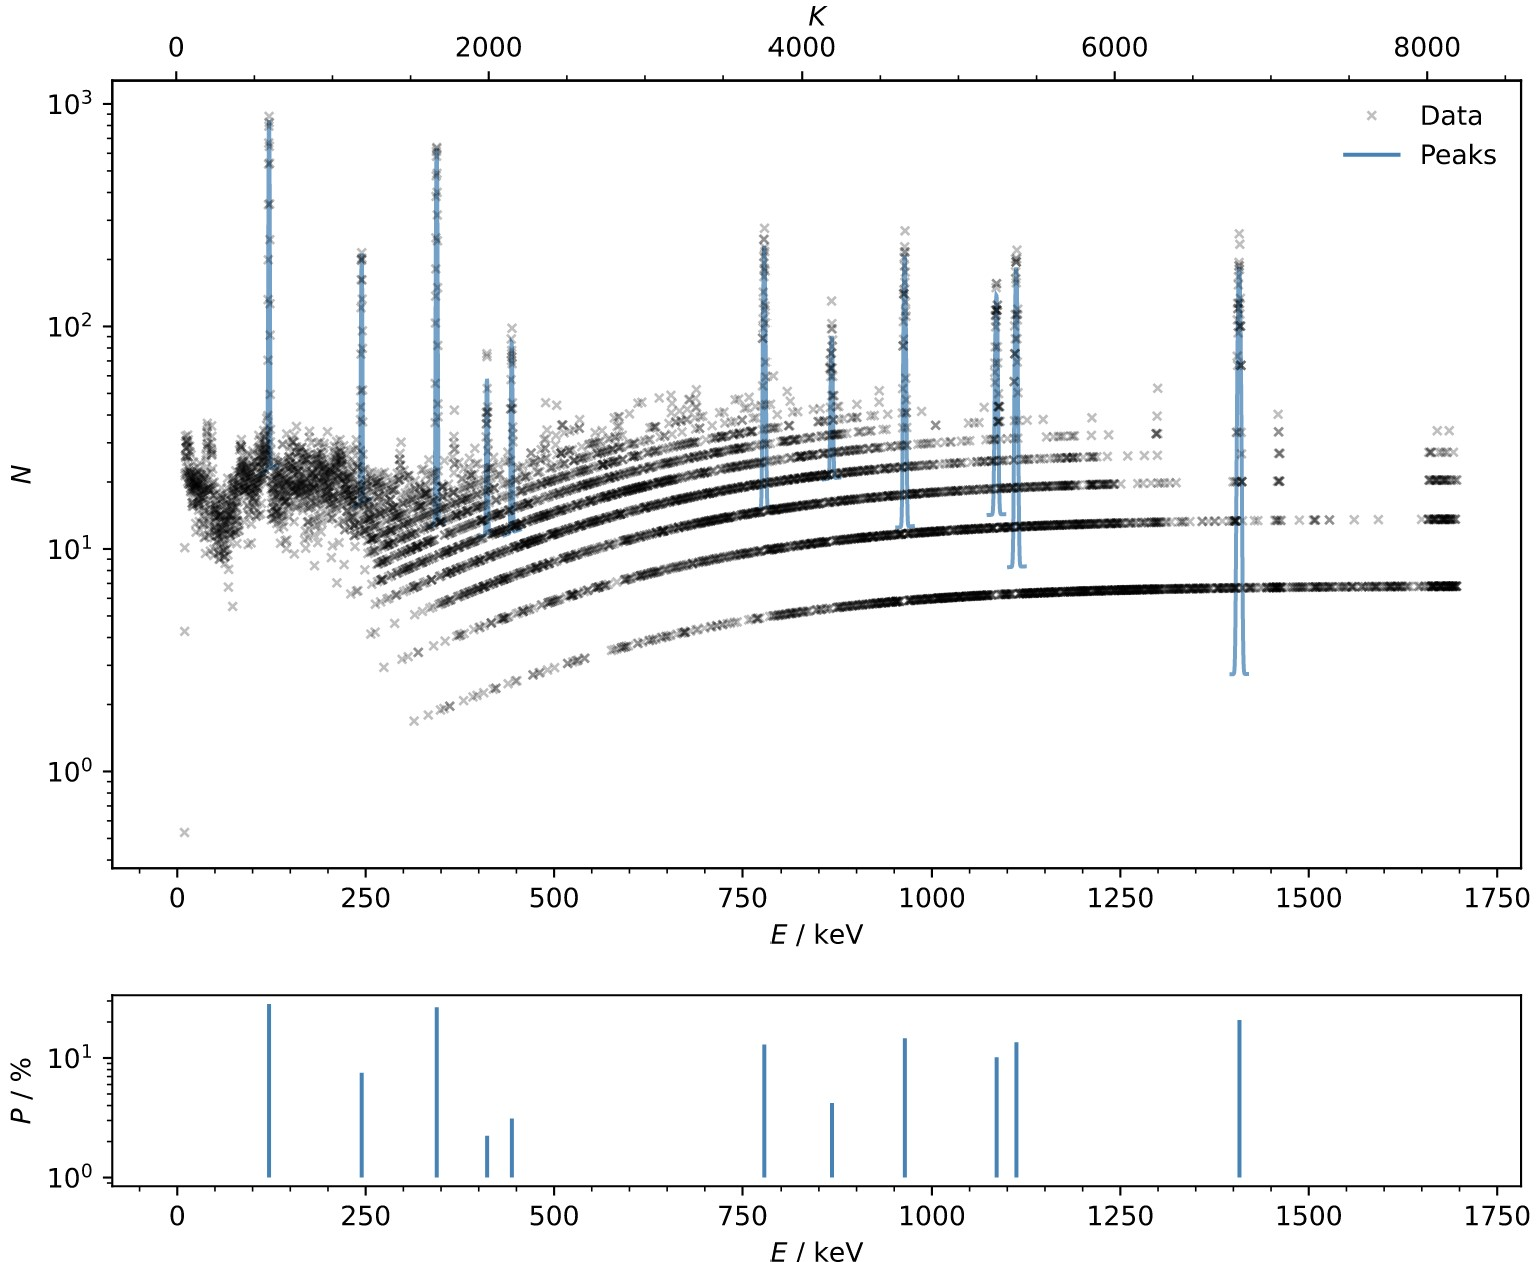
\includegraphics[width=0.9\textwidth]{content/plots/plot6.jpg}
   \caption{korrigiertes Gammaspektrum des Eu-152 Strahlers.}
    \label{fig:plot6}
\end{figure}

\subsection{Untersuchung eines monochromatischen Gamma Spetrums}
\label{sec:untersuchung gamma spektrum}

Für den ersten Aufgabenteil dieses Abschnittes wurde ein Cs-137 Strahler vermessen.
Das dazugehöroge Spektrum ist in der Abbildung \ref{fig:plot7} zu sehen.

\begin{figure}[H]
    \centering
    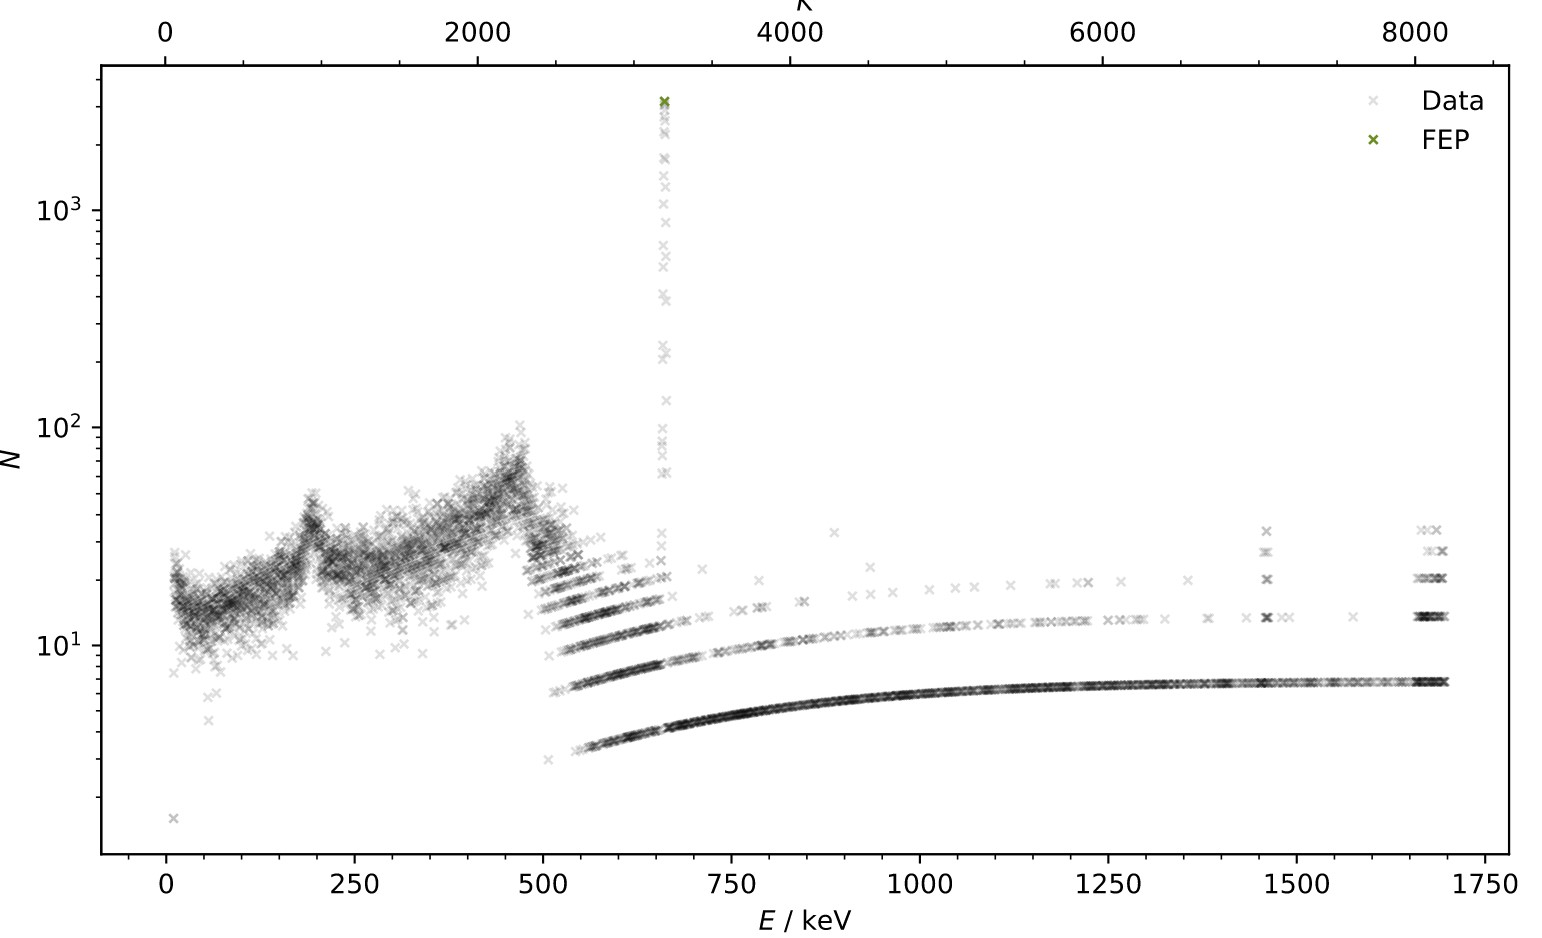
\includegraphics[width=0.9\textwidth]{content/plots/plot7.jpg}
    \caption{Das Spektrum eines monochromatischen Cs-137 Strahlers.}
    \label{fig:plot7}
\end{figure}

Abgelesen werden kann das Compton Kontinuum., die Compton-Kante, der Rückstreupeak und der Photopeak.
Mit Hilfe eines Gaußkurve, welche an den Photopeak gelegt wird,soll die Anzahl der Impulse bestimmt werden.
Indem dann die Halbwertsbreite und die Zehntelwertsbreite bestimmt wird, kann der Fit überprüft werden.
Die Energie des Photopeakswird mittels dem SciPy Paket find-peaks ermittelt.
Die Gauß-Kurve hat die Form 
\begin{equation}
    f(x) = b + \frac{N}{\sqrt{2 \pi \sigma^2}} \exp{-\frac{\left(x-\mu \right)^2}{2\sigma^2}}.
    \label{eqn:gauss}
\end{equation}
 
Für die Parameter ergeben sich folgende Werte
\begin{align*}
    b &=    \num{7.739+- 2.241} \\
    m &=  \num{661.182+- 0.004} \\
    s &=    \num{0.944+-0.004} \\
    N &= \num{7624.639+-27.994}.
\end{align*}

Der Photopeak mit der Gaußkurve ist in Abbildung \ref{fig:plot8} dargestellt.

\begin{figure}[H]
    \centering
    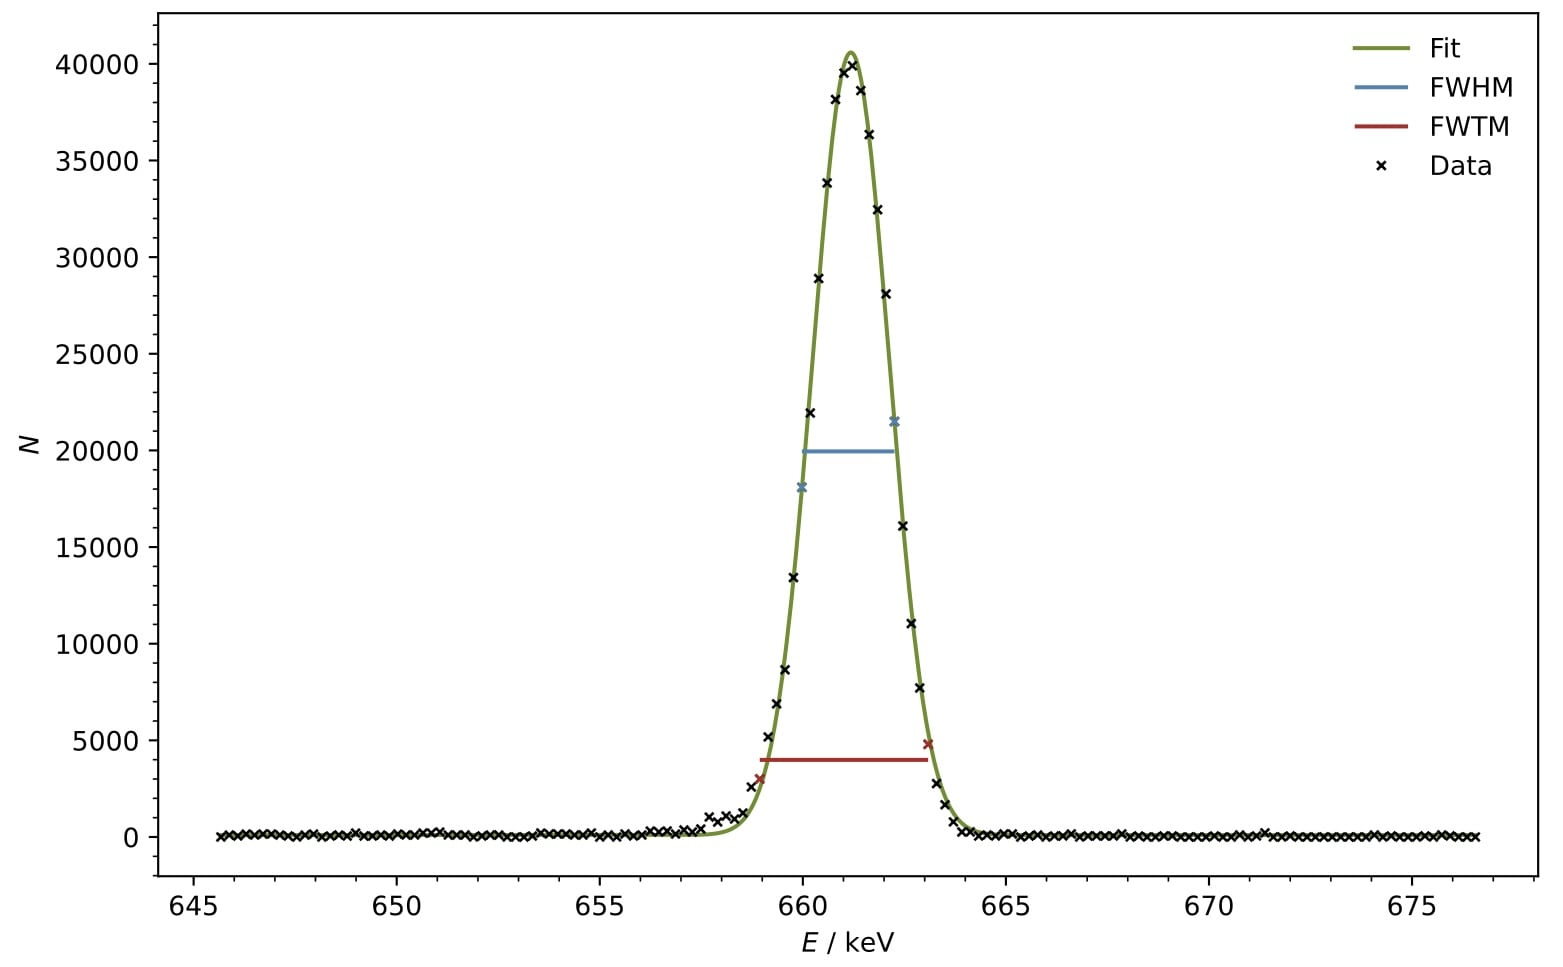
\includegraphics[width=0.9\textwidth]{content/plots/plot8.jpg}
    \caption{Full Energy Peak des Cs-137 Strahlers.}
    \label{fig:plot8}
\end{figure}

Aus der Umstellung der Gaußfunktion folgen die theorethischen Werte
\begin{align*}
 f_{\text{fwhm}} &= 2 \sqrt{2 \ln{2}} \sigma \\
 f_{\text{fwtm}} &= 2 \sqrt{2 \ln{10}} \sigma.
\end{align*}
Für das Verhältnis der Zehntelwertsbreite und der halbwertsbreite ergibt sich dann
\begin{equation*}
  \frac{f_{\text{fwhm}}}{f_{\text{fwtm}}} = \sqrt{\frac{\ln{10}}{\ln{2}}} \approx \num{1.823}
\end{equation*}

Aus der Messung wurden die charakteristischen Breiten durch die nächstgelegenden Messpunkte angenähert. 
\begin{align*}
    f_{\text{fwhm}} &\approx \qty{2.28}{\kilo\eV}\\
    f_{\text{fwtm}} &\approx \qty{4.15}{\kilo\eV}.
\end{align*}
Das Verhältnis beträgt
\begin{equation*}
    \frac{f_{\text{fwhm}}}{f_{\text{fwtm}}} \approx \num{1.818}.
\end{equation*}
   